\documentclass[a4paper]{article}

%% Language and font encodings
\usepackage[english]{babel}
\usepackage[utf8x]{inputenc}
\usepackage[T1]{fontenc}

%% Sets page size and margins
\usepackage[a4paper,top=3cm,bottom=2cm,left=3cm,right=3cm,marginparwidth=1.75cm]{geometry}

%% Useful packages
\usepackage{amsmath}
\usepackage{graphicx}
\usepackage{subfig}
\usepackage[colorinlistoftodos]{todonotes}
\usepackage[colorlinks=true, allcolors=blue]{hyperref}
\usepackage{float}

\title{MCAA Mini Project: Team Ergotic Pain}
\author{Ignacio Aleman, Ahmed Furkan Özkalay, Sidak Pal Singh\\\texttt{ignacio.aleman@epfl.ch}, \texttt{ahmed.ozkalay@epfl.ch}, \texttt{sidak.singh@epfl.ch}}

\begin{document}
\maketitle

\vspace*{\fill}
\section{Introduction}

Consider the following learning problem. One has a set of M “patterns” modeled as N-dimensional vectors $x_\mu \in R^{N}, \mu = 1, . . . , M$. Each pattern belongs to one of two “classes” $y_\mu \in \{−1, +1\}$. One would like to “learn” a vector of “weights” $\underline{w}$ such that the following constraints are satisfied (or at least the number of errors is minimized):
$$y_\mu = sign(\underline{w} \cdot \underline{x}_\mu), \mu = 1, . . . , M$$
Geometrically, w corresponds to a vector perpendicular to a hyperplane that separates/classifies the patterns into two classes. The aim is to minimize the total cost or energy function, defined as
$$E(w) = \sum_{\mu=1}^{M}(y_\mu − sign(\underline{w} \cdot \underline{x}_\mu))^2$$
which counts the number of misclassification for a vector $\underline{w}$.
For $\underline{w} \in R^{N}$, this model is called the binary perceptron (because there are two classes) and for $\underline{w} \in \{−1, +1\}^{N}$ it is called the Ising perceptron because the weights can be seen as Ising spins and E($\underline{w}$) as an “Ising type” Hamiltonian or energy function. One is interested in particular in the regime where the ratio $\alpha = \dfrac{M}{N}$ is fixed and $N$, $M$ are both large (in theory, $N$, $M \to\infty$).

In the teacher-student scenario, a “teacher” has a separating plane $w^{∗}$ and generates a set of patterns $x_\mu$, as well as their class labels $y_\mu =$ sign($w \cdot x_\mu)$. The “student” has access to the pairs $(y_\mu, x_\mu)$ called the “training set” and her task is to find $w^{*}$. We assume that $w^{*} \in \{-1, +1\}^{N}$ has i.i.d. Ber($1/2$) components and that $x_\mu$ have i.i.d. Gaussian components with mean zero and unit variance. Of course, in this case, $w^{*}$ is a minimizer of $E(w)$ and $E(w^{*}) = 0$. One expects that for $\alpha$ large enough, the student should be able to learn $w^{*}$, while if $\alpha$ is too small, then she might find a wrong solution.

Desperate to please his teacher, the student decides to set up an MCMC chain by looking at a finite temperature version of the problem. In what follows the said student and his companions shall try to shed more light into this problem as they explore the behavior of energy as well as other relevant metrics by letting the various parameters vary.

\newpage
\section{Results of exploration}

In this section we will examine different values of MCMC iterations for different alpha and beta values. Energy vs time, normalized energy vs alpha and overlap vs alpha will be examined in following subsections.

\subsection{Energy vs Time}
The number of dimension is set to 40. For each alpha and beta combination, the results are averaged for 100 MCMC runs. The values of alpha are 0.5, 2.5 and 5, which means the values of M are 20, 100 and 200. The values of beta are 0.6, 1 and 1.4. MCMC iterations are stopped if energy becomes 0 or number of iterations reach 5000. The energy vs time plot for different alpha and beta combinations are given below.

\begin{figure}[H]
\centering
\includegraphics[width=1\textwidth]{part1_tight.png}
\caption{\label{fig:part1}Energy vs time for different alpha and beta values}
\end{figure}

For each case energy goes down as time progresses as expected (otherwise using MCMC to minimize energy function would not make sense at all). For small alpha (alpha = 0.5), increasing beta gives better performance; smaller energy and faster convergence. The reason is as beta decreases MCMC moves more randomly as temperature is high in a sense. However, there are already various solutions minimizing the energy so exploring different states slows down the convergence and degrades performance. Similar pattern cannot be really seen for alpha = 2.5 and alpha = 5, for those cases curves are very similar for different values of alpha. When one fixes values of beta and compares the curves for different values of alpha (i.e. increase number of samples), MCMC converges faster to a better solution (with a low energy). This can be interpreted as following, ones the number of examples are higher then it is easier to learn a better omega which minimizes the energy. But note that, as alpha increases energy also increases for fixed beta. The reason is these values are not normalized. Once these values are divided by alpha, then fair comparison would be possible.

\subsection{Normalized Energy vs Alpha}
The number of dimension is set to 40. For each alpha and beta combination, the results are averaged for 100 MCMC runs. The values of alpha are 0.5, 1, 1.5, 2, 2.5, 3, 3.5, 4, 4.5 and 5, which means the values of M are 20, 40, 60, 80, 100, 120, 140, 160, 180 and 200. The values of beta are 0.4, 0.6, 0.8, 1, 1.2, 1.4 and 1.6. We examine the normalized energy at 500th time step. The normalized energy vs alpha plot for different beta combinations are given below.

\begin{figure}[H]
\centering
\includegraphics[width=1\textwidth]{part2_tight.png}
\caption{\label{fig:part2}Normalized Energy vs alpha for different beta values}
\end{figure}

For very small values of beta (for example, beta = 0.1, 0.3, 0.7), MCMC in a sense moves very randomly as temperature is high. Thus, energy is not minimized very much, although as alpha increases performance also increases. For higher values of beta (beta = 1, 1.5), energy is consistently low across all alpha values. It begins very small for alpha = 0.5 and beta = 1.5 as for small alpha values there are multiple solutions that minimize the energy (because there are smaller number of patterns that one has to predict), then for increasing alpha the problem becomes harder and energy increases. But when alpha further increases since there are lots of patterns that one can learn from, energy further decreases. One importance observation is that, for higher values of alpha one should not set beta very small or very high. Because the former tends to over explore whereas the latter tends to under explore. For moderate values of beta, one can balance exploration for the case with high alpha values.

\subsection{Overlap vs Alpha}
The number of dimension is set to 40. For each alpha and beta combination, the results are averaged for 100 MCMC runs. The values of alpha are 0.4, 0.6, 0.8, 1, 1.2, 1.4 and 1.6, which means the values of M are 20, 40, 60, 80, 100, 120, 140, 160, 180 and 200. The values of beta are 0.1, 0.3, 0.7, 1 and 1.5. MCMC iterations are stopped if energy becomes 0 or number of iterations reach 5000. The normalized energy vs alpha plot for different beta combinations are given below.

\begin{figure}[H]
\centering
\includegraphics[width=1\textwidth]{part3_tight.png}
\caption{\label{fig:part3}Overlap vs alpha for different beta values}
\end{figure}

Using MCMC algorithm we try to minimize energy function. However, for alpha being small (which means number of examples per dimension is smaller) there might be different state spaces which minimize the energy. MCMC algorithm might find one of these which would give very low energy with small overlap with teacher's solution. Indeed, for all values of beta we see that as alpha increase overlap also increases. The reason is teacher's solution becomes the only solution that minimizes the energy function and when MCMC tries to minimize energy it also becomes more and more similar to teacher's solution. The curve is significantly different for different values of beta as expected. For small beta values, temperature is high which corresponds to more random (i.e. more exploratory) moves. In that case overlap is smaller for small values of alpha. On the contrary, when alpha is higher small beta performs very well (in fact best performing two cases are for 2 smallest betas). For high values of beta, performance is consistently better for small values of alpha, but for high values of alpha performance is strictly worse. The conclusion would be for small datasets (i.e. alpha is small) high betas would find better solution (higher overlap with teacher's omega) as it tends to not explore and as alpha increase (having more samples) having small beta and exploring state space gives high performance in terms of having higher overlap and thus approximating teacher's omega better.

\newpage
\section{Simulated Annealing}
While the name and inspiration of this concept comes from metallurgy, it is essentially a method to find a good solution to an optimization problem, where typically the optimization landscape has many local optima. We use simulated annealing here to reach a state of low energy which is as close as possible to the teacher's vector, in context of Markov Chain Monte Carlo.

\subsection{Grid Search}
In order to find the best set of parameters for simulated annealing, we carry out a grid search over a selected range of values for each of them. In particular, we set \textit{N\_values} to $[40, 60, 75, 100]$, \textit{beta\_values} to $[0.1, 0.3, 0.4, 0.7, 0.9]$, \textit{pace\_values} to $[1.0002, 1.001, 1.002]$, and \textit{schedule\_values} $[1, 10]$. In other words, the above denote the range of values for dimension, initial beta, pace (with which beta is increased) and schedule of this pace (i.e. after how many iterations to increase the pace), respectively. Since, with increasing \textit{N}, the problem has a larger state space, we decrease the number of runs accordingly. Specifically, we set the number of runs to $[50, 40, 30, 20]$ for the corresponding \textit{N\_values}.

Note that running such a grid search becomes intractable on a normal laptop/computer, and hence we run it in parallel with 48 cores on one of the machines in ic\_cluster.

Note also that we have "highly" optimized the code; As suggested, we simplified the difference in energy as indeed once $E(\omega)$ is computed, $E(\omega^{\dagger})$ is cheap to compute. We have also kept computation to a minimum by storing variables which might be reused. The implementation of these optimizations can be seen in the code.

\subsection{Analysis}
Here, we do a comparative analysis of the effect due to each of the parameters. In this analysis, the running example will be of the case when $N$ is $100$ and we will try to understand the effect of (initial) value of beta, pace, and schedule. We put our attention on N = 100 since we observe similar results for different values for N; In the appendix plots for the same experiments done for N = 75 are shown as an example of the similar trends observed for a different N.\\

\textbf{General Trends}: We observe that in general, the overlap per alpha grows roughly linearly with alpha (i.e. increasing number of samples, $M$, for a fixed $N$), and reaches $1$ around alpha equal to $4$ or $5$. [Figure 4.] Next, the normalized energy per alpha for most of the explored grid points is roughly concave with low energy values for small alpha (like $1$), increasing until alpha is around 2 and then rapidly decaying. Though for a particular setting of parameters, we also observe an almost monotonically decaying normalized energy curve. [Figure 4.] \\

\begin{figure}[H]
    \centering
    {{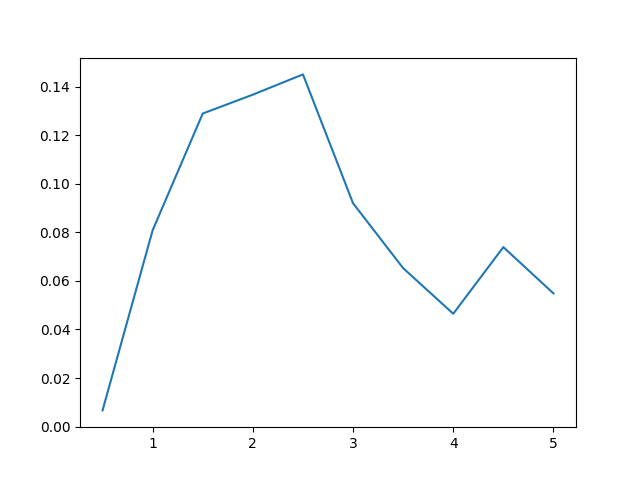
\includegraphics[width=5cm]{normalized_energies_per_alpha.png} }}%
    \qquad
    {{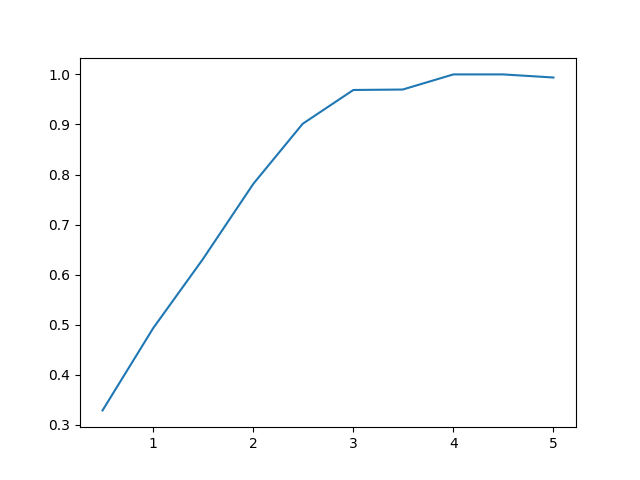
\includegraphics[width=5cm]{overlap_per_alpha.png} }}%
    \caption{Normalized energy and overlap as a function of alpha. Fixed N = 100, and for various initial beta starting points.}%
    \label{fig:example}%
\end{figure}

\textbf{Effect of schedule}: When the schedule is 10 (i.e. the beta is increased after every 10 iterations), this implies that the algorithm is able to explore more and as a result has lower normalized energy for moderate to large alpha (more specifically from around 2 to 5). [Figure 5.] But, for the case when alpha is low (like around 1), there are multiple solutions and it seems better to go direct to solution and explore less (as with $schedule = 1$). As a result, we can also observe in the overlap per alpha graph that when for low alpha and $schedule = 1 $, the overlap is more while in the case for larger alpha and $schedule = 10$, the overlap dominates and essentially becomes 1. [Figure 5.] \\

\begin{figure}[H]
    \centering
    {{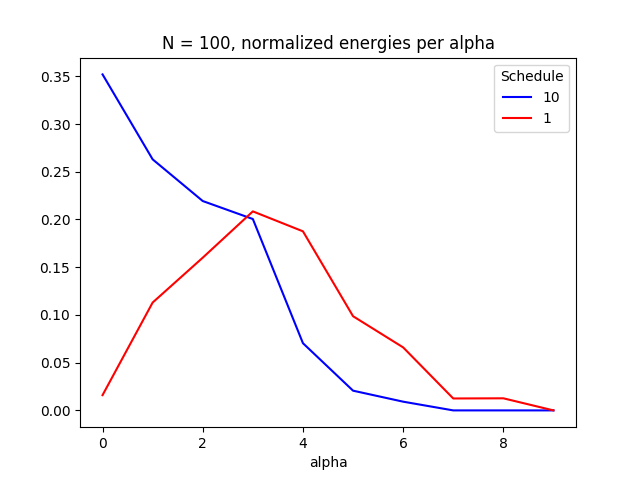
\includegraphics[width=5cm]{normalized_energies_per_alpha_schedule.png} }}%
    \qquad
    {{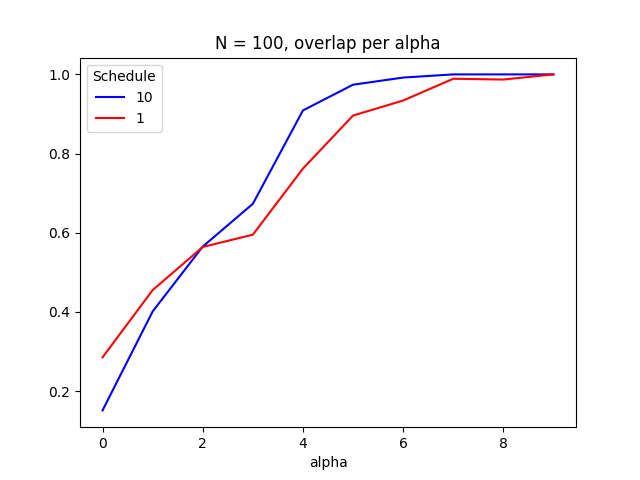
\includegraphics[width=5cm]{overlap_per_alpha_schedule.png} }}%
    \caption{Normalized energy and overlap as a function of alpha. Fixed N = 100, and for Schedule's 1 and 10.}%
    \label{fig:example}%
\end{figure}

\textbf{Effect of initial beta}:  In this analysis, the values of initial beta which are compared against are $[0.1, 0.3, 0.4, 0.7]$.  Schedule is kept equal to $10$ and pace as $1.0002$. We observe that for alpha varying from $0.5$ to $2$, $beta=0.7$ leads to fastest convergence. [Figure 6.] Next, $beta=0.1$ generally takes more iterations to converge, which is expected as it does more exploration (highest temperature). For $alpha$ greater than $2$ until $5$, $beta=0.4$ always dominates. An important point to remark is that these observations remain consistent across the value of $N$, and we get similar plots for $N=75$ and $N=100$. Lastly, from the normalized energy per alpha and the overlap per alpha graphs [Figure 4.], we notice that $beta=0.3$ and $beta=0.4$ perform similar and outperform other values of $beta$ for most of the values for $alpha$. [Figure 6.]\\
\vspace{0.5cm}
\begin{figure}[H]
\centering
\includegraphics[width=1\textwidth]{N_100.png}
\caption{\label{fig:part1}Energy vs time for different alpha and initial beta values}
\end{figure}
\newpage
\textbf{Effect of pace}: The pace essentially dictates how fast we settle for what seems like a good solution. Indeed, a fast pace is equivalent to a fast temperature drop, and hence we should expect that while we might reach low energies quickly, we will as a consequence possibly miss out on better local (or hopefully global) energies. What we see in practice (for N=100) seems to support this hypothesis. For alpha between 0.5 and 2 there seems to be no benefit in using a slower pace [Figure 7.] (We arbitrarily chose to limit iteration time to 100000, we thus limit ourselves to this time window; Note that for the slower pace in blue the energy still appears to decrease). For alpha over 2 we can see the aforementioned trade off cashing in: In plots 4, 5 and 6 (of figure 7) we observe that a slower pace (blue) has allowed us to achieve lower energies which could not be found as we get stuck too quickly as a consequence of the quicker pace (red and green). We would like to point out that this is similar in flavor to the approach taken in the multi-arm bandit problem where the trade off is between exploration and exploitation. The higher temperature regime is equivalent to exploration, and lowering it is akin to getting the best location among the explored places (If we were to keep track of the best energy found then this would be the case).

\vspace{1cm}

\begin{figure}[H]
\centering
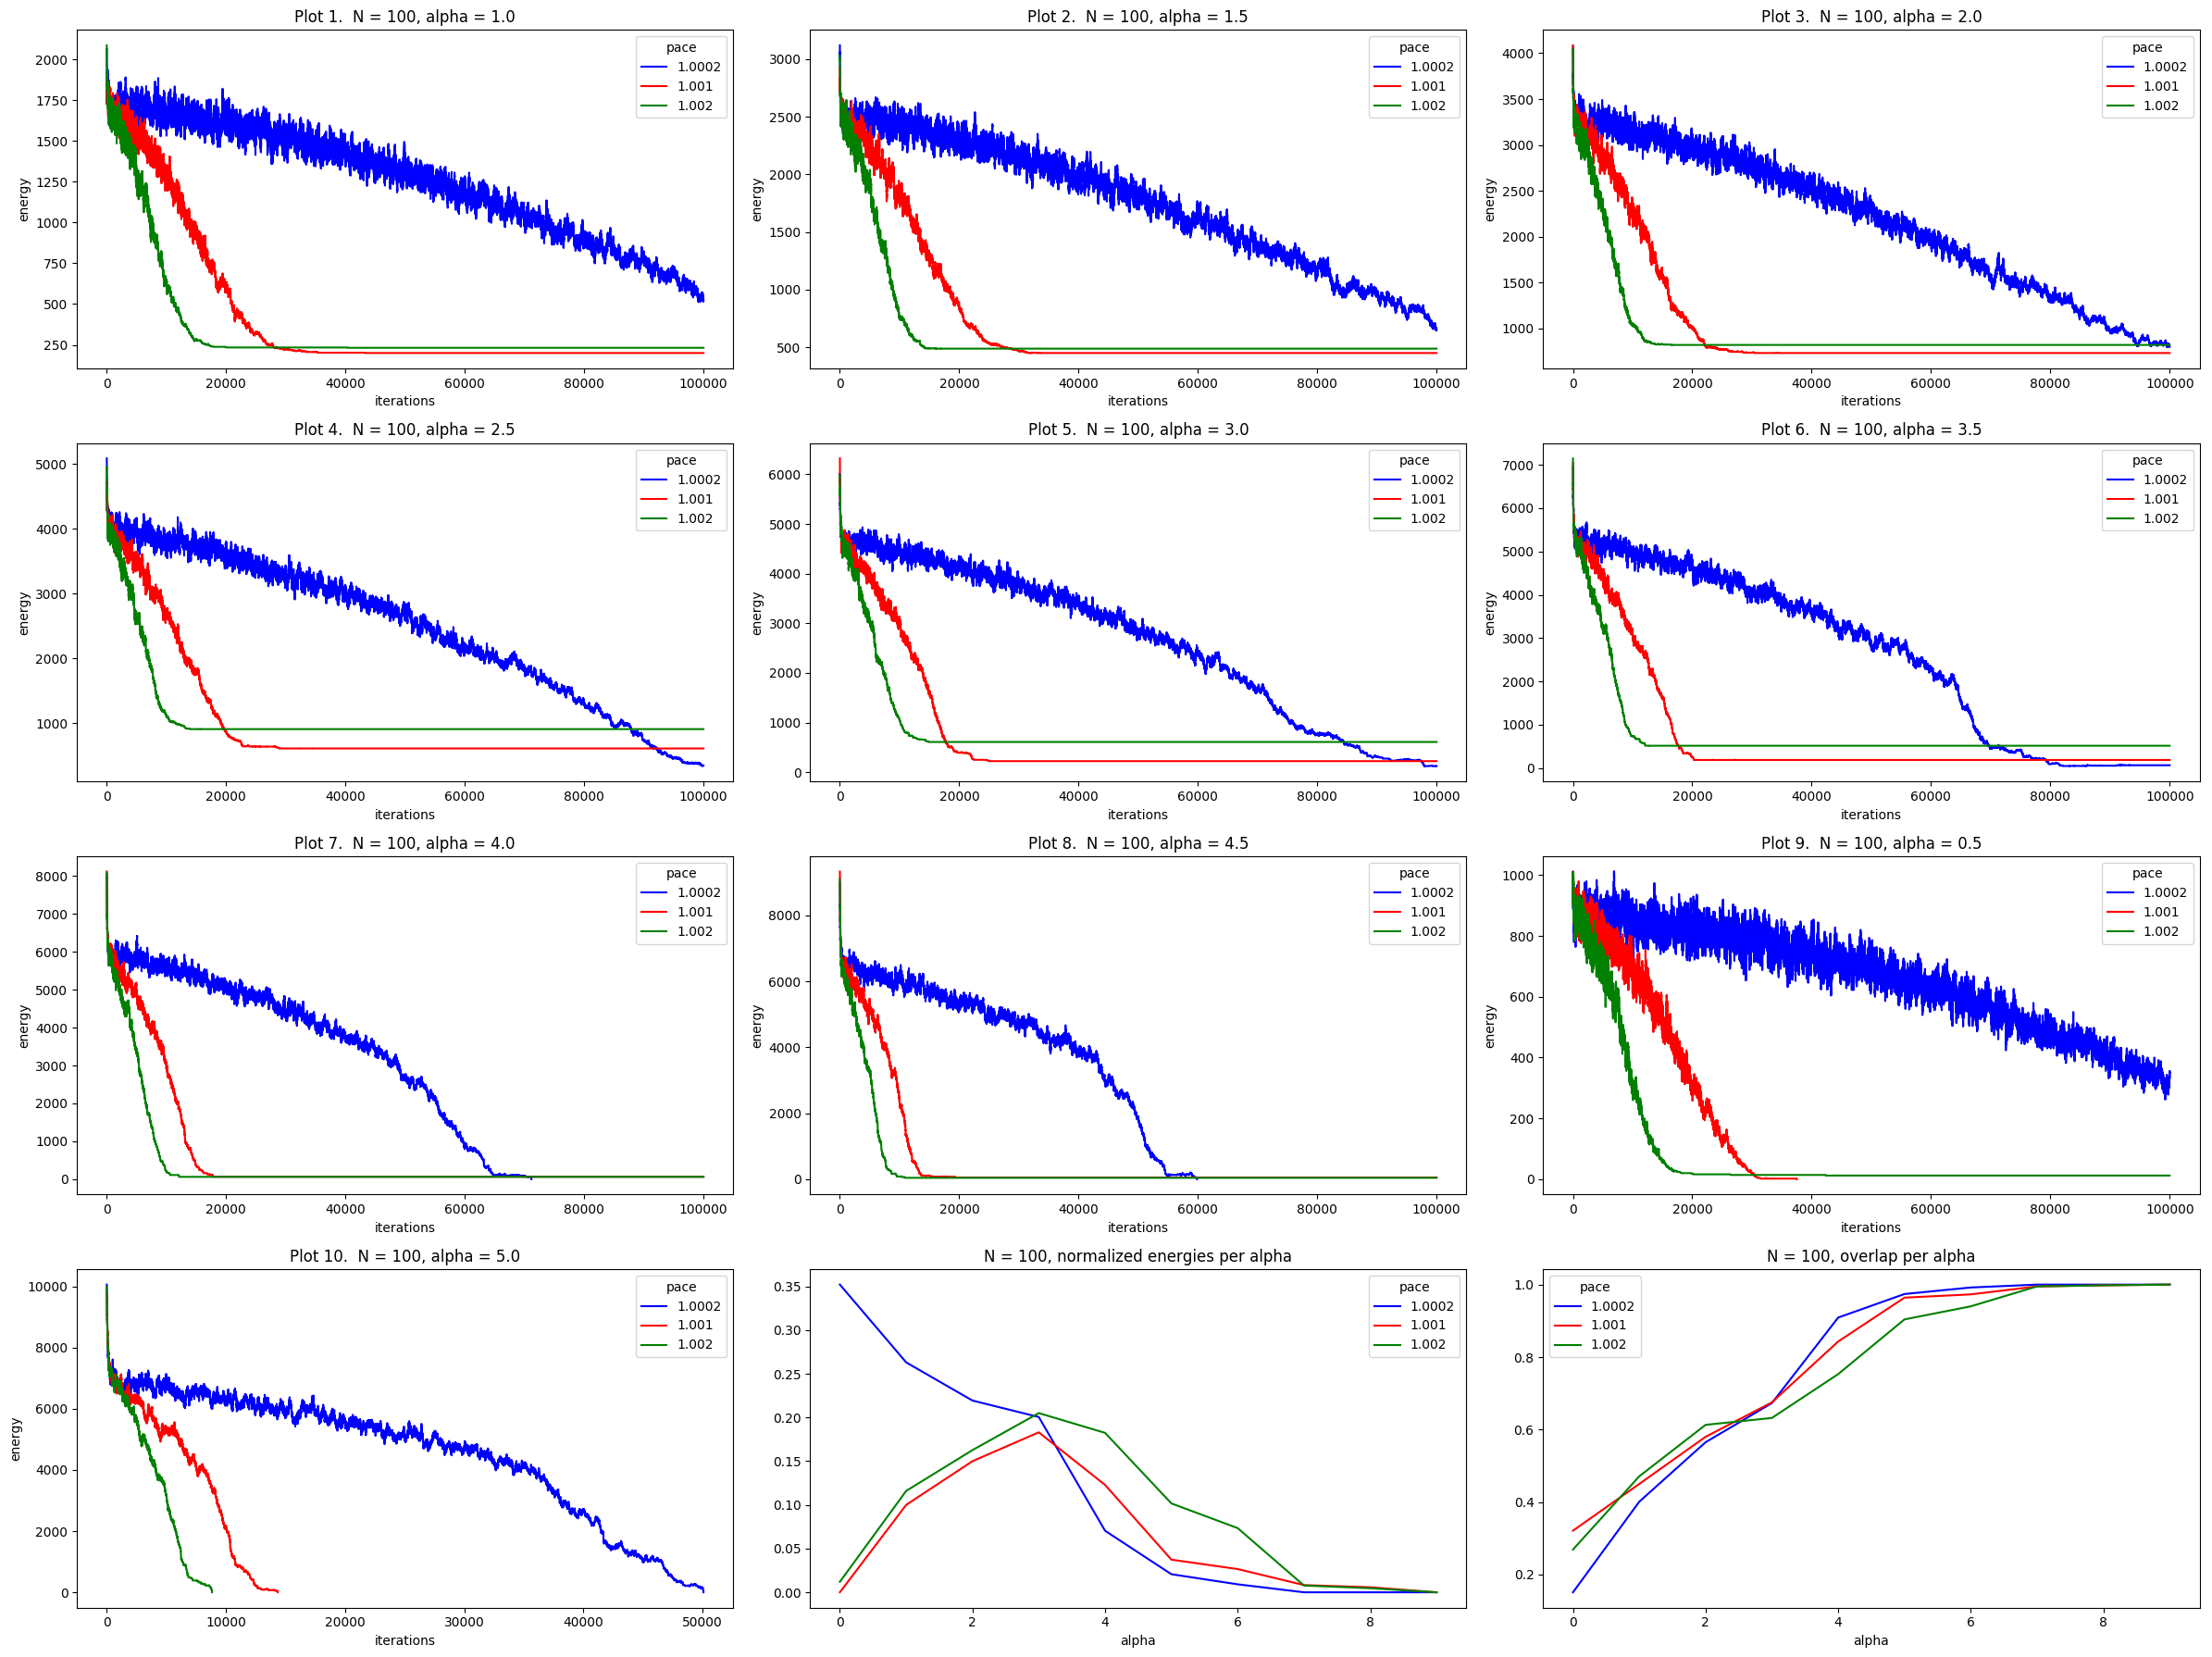
\includegraphics[width=1\textwidth]{pace.png}
\caption{\label{fig:part1}Energy vs time for different alpha and pace rates}
\end{figure}

\newpage
\appendix
\section{Appendices}

\begin{figure}[H]
\centering
\includegraphics[width=1\textwidth]{N_75.png}
\caption{\label{fig:part1}Energy vs time for different alpha and initial beta values. This is the same as figure 6 and 5 but with N = 75.}
\end{figure}

\end{document}
